\icode[magenta]{E-MM-CA-L4-261014-002}
如图所示，地面上静止地放置着质量为\(M\)的木块，其底部为平面。上部有截面为半圆的凹槽，半	径为\(R\)，质量为\(m\)的小球从最高处静止下滑。设各种摩擦及阻力均可略。试求：
\begin{enumerate}
	\item 在小球\(m\)下滑过程中，\(m\)的绝对速度\(v\)，\(M\)的绝对速	度\(v_M\)以及\(m\)的相对速度\(\mu\)随小球位置\(\theta\)的变化规律。
	\item 小球\(m\)在最低点时给木块\(M\)的压力。
	\item 问：小球\(m\)速度是否存在最大值？若存在，最大值在哪取到？
	\item 求任意\(\theta\)时球和槽之间的弹力\(N(\theta)\)。
	\item 求\(m\)的轨迹。
\end{enumerate}

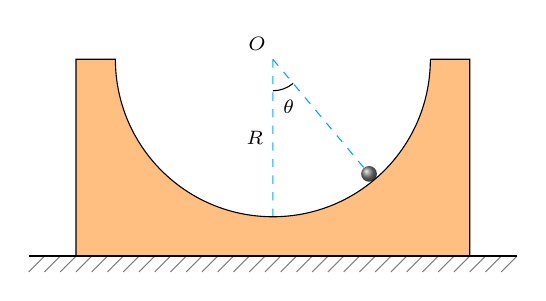
\begin{tikzpicture}[font=\scriptsize]
	\draw[dashed,cyan] (0,0)--node[left,black]{\(R\)}(0,-2) (0,0)--(-50:2);
	\shade[ball color=gray] (-50:1.9) circle(.1);
	\draw (0,-.4) arc(-90:-50:.4);
	\draw[fill=orange!50] (2,0) arc(0:-180:2)--(-2.5,0)--(-2.5,-2.5)--(2.5,-2.5)--(2.5,0)--(2,0);
	\node at(.2,-.6){\(\theta\)};
	\node at(-.2,.2){\(O\)};
	\foreach \x in {-3.1,-2.9,...,3.1}
		\draw[gray] (\x,-2.7)--++(.2,.2);
	\draw[thick] (-3.1,-2.5)--(3.1,-2.5);
\end{tikzpicture}